% !TeX root = RJwrapper.tex
\title{Timing Rayleigh Quotient minimization in R}
\author{by John C. Nash}

\maketitle

\abstract{%
This vignette is simply to record the methods and results for timing various Rayleigh Quotient minimizations with R using different functions and different ways of running the computations, in particular trying Fortran subroutines and the R byte compiler. It has been updated from a 2012 document to reflect changes in R and its packages that make it awkward to reprocess the original document on newer computers.
}

\subsection{The computational task}\label{the-computational-task}

The maximal and minimal eigensolutions of a symmetric matrix \(A\) are extrema of the Rayleigh Quotient

\[ R(x) =  (x' A x)  / (x' x) \]

We could also deal with generalized eigenproblems of the form

\[A x = e B x\]

where \(B\) is symmetric and positive definite by using the Rayleigh Quotient (RQ)

\[ R_g(x) =  (x' A x)  / (x' B x) \]

In this document, \(B\) will always be an identity matrix, but some programs we test
assume that it is present.

Note that the objective is scaled by the parameters, in fact by by their
sum of squares. Alternatively,
we may think of requiring the \textbf{normalized} eigensolution, which is given as

\[ x_{normalized} = x/sqrt(x' x) \]

\subsection{Timings and speedups}\label{timings-and-speedups}

In R, execution times can be measured by the function \texttt{system.time\},\ and\ in\ particular\ the\ third\ element\ of\ the\ object\ this\ function\ returns.\ \ However,\ various\ factors\ influence\ computing\ times\ in\ a\ modern\ computational\ system,\ so\ we\ generally\ want\ to\ run\ replications\ of\ the\ times.\ The\ R\ packages\ \textbackslash{}pkg\{rbenchmark\}\ and\ \textbackslash{}pkg\{microbenchmark\}\ can\ be\ used\ for\ this.\ I\ have\ a\ \ preference\ for\ the\ latter.\ However,\ to\ keep\ the\ time\ to\ prepare\ this\ vignette\ with\ \textbackslash{}pkg\{Sweave\}\ or\ \textbackslash{}pkg\{knitR\}\ reasonable,\ many\ of\ the\ timings\ will\ be\ done\ with\ only}system.time\}.

There are some ways to speed up R computations.

\begin{itemize}
\tightlist
\item
  The code can be modified to use more efficient language structures. We
  show some of these below, in particular, to use vector operations.
\item
  We can use the R byte code compiler by Luke Tierney, which has been
  part of the R distribution since version 2.14.
\item
  We can use compiled code in other languages. Here we show how Fortran
  subroutines can be used.
\end{itemize}

\subsection{Our example matrix}\label{our-example-matrix}

We will use a matrix called the Moler matrix \cite[Appendix 1]{cnm79}.
This is a positive definite
symmetric matrix with one small eigenvalue. We will show a couple of
examples of computing the small eigenvalue solution, but will mainly
perform timings using the maximal eigenvalue solution, which we will
find by minimizing the RQ of (-1) times the matrix. (The eigenvalue
of this matrix is the negative of the maximal eigenvalue of the
original, but the eigenvectors are equivalent to within a scaling
factor for non-degenerate eigenvalues.)

Here is the code for generating the Moler matrix.

\begin{verbatim}
molermat<-function(n){
   A<-matrix(NA, nrow=n, ncol=n)
   for (i in 1:n){
      for (j in 1:n) {
          if (i == j) A[i,i]<-i
          else A[i,j]<-min(i,j) - 2
      }
   }
   A
}
\end{verbatim}

However, since R is more efficient with vectorized code, the following routine by
Ravi Varadhan should do much better.

\begin{verbatim}
molerfast <- function(n) {
# A fast version of `molermat'
  A <- matrix(0, nrow = n, ncol = n)
  j <- 1:n
  for (i in 1:n) {
    A[i, 1:i] <- pmin(i, 1:i) - 2
  }
  A <- A + t(A)
  diag(A) <- 1:n
  A
}
\end{verbatim}

\subsubsection{Time to build the matrix}\label{time-to-build-the-matrix}

Let us see how long it takes to build the Moler matrix of different sizes.
In 2012 we used the byte-code compiler, but that now seems to be active by
default and NOT to give worthwhile improvements.
We also include times for the \texttt{eigen()} function that computes
the full set of eigensolutions very quickly.

\begin{verbatim}
#> Loading required package: microbenchmark
\end{verbatim}

\begin{verbatim}
#>      n buildi   osize eigentime bfast
#> 1   50   4629   20216       878   779
#> 2  100   5978   80216      2057   625
#> 3  150  10137  180216      3957  1075
#> 4  200  16038  320216      5804  1368
#> 5  250  24332  500216      8499  1835
#> 6  300  34353  720216     11155  2383
#> 7  350  45956  980216     14401  3042
#> 8  400  58746 1280216     19217  3838
#> 9  450  77465 1620216     24626  4295
#> 10 500  91166 2000216     31533  7817
\end{verbatim}

\begin{verbatim}
#> buildi - interpreted build time
\end{verbatim}

\begin{verbatim}
#> osize - matrix size in bytes; eigentime - all eigensolutions time
\end{verbatim}

\begin{verbatim}
#> bfast - interpreted vectorized build time
\end{verbatim}

\begin{verbatim}
#> Times converted to milliseconds
\end{verbatim}

It does not appear that the compiler has much effect, or else it is being automatically invoked.

We can graph the times. The code, which is not
echoed here, also models the times and the object size
created as almost perfect quadratic models in \texttt{n}. However,
the vectorized code is much, much faster, and the byte code
compiler does not appear to help.

\begin{verbatim}
#> 
#> Call:
#> lm(formula = ti ~ n + n2)
#> 
#> Residuals:
#>     Min      1Q  Median      3Q     Max 
#> -1409.0  -353.8  -126.0   161.3  2358.6 
#> 
#> Coefficients:
#>               Estimate Std. Error t value Pr(>|t|)    
#> (Intercept) 3815.50246 1319.58797   2.891   0.0233 *  
#> n            -13.42906   11.02231  -1.218   0.2626    
#> n2             0.38189    0.01953  19.554 2.28e-07 ***
#> ---
#> Signif. codes:  0 '***' 0.001 '**' 0.01 '*' 0.05 '.' 0.1 ' ' 1
#> 
#> Residual standard error: 1122 on 7 degrees of freedom
#> Multiple R-squared:  0.999,  Adjusted R-squared:  0.9987 
#> F-statistic:  3358 on 2 and 7 DF,  p-value: 3.642e-11
\end{verbatim}

\begin{verbatim}
#> 
#> Call:
#> lm(formula = tf ~ n + n2)
#> 
#> Residuals:
#>      Min       1Q   Median       3Q      Max 
#> -1110.72  -178.17    49.68   238.83   954.48 
#> 
#> Coefficients:
#>              Estimate Std. Error t value Pr(>|t|)   
#> (Intercept) 1292.0116   702.8706   1.838  0.10863   
#> n             -8.8585     5.8710  -1.509  0.17507   
#> n2             0.0400     0.0104   3.845  0.00633 **
#> ---
#> Signif. codes:  0 '***' 0.001 '**' 0.01 '*' 0.05 '.' 0.1 ' ' 1
#> 
#> Residual standard error: 597.6 on 7 degrees of freedom
#> Multiple R-squared:  0.9424, Adjusted R-squared:  0.9259 
#> F-statistic: 57.25 on 2 and 7 DF,  p-value: 4.589e-05
\end{verbatim}

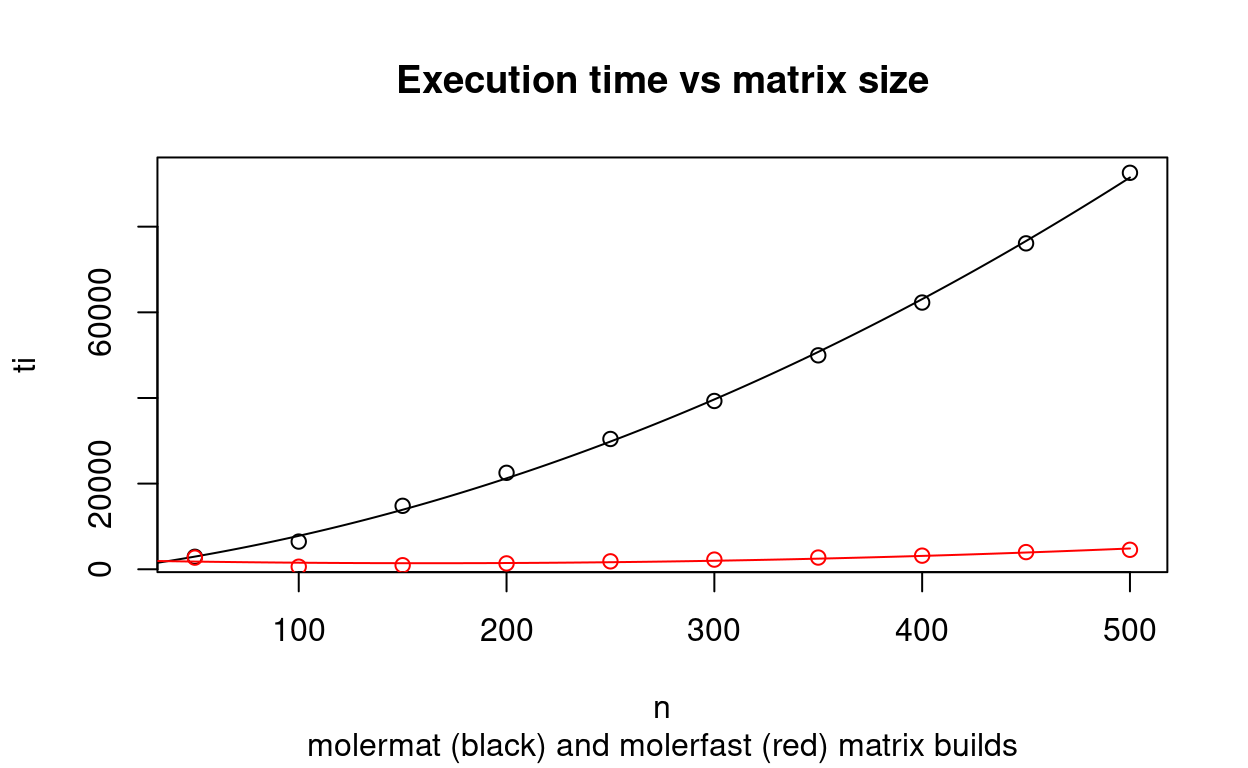
\includegraphics{RQtimes_files/figure-latex/drawtime1-1.pdf}

\begin{verbatim}
#> Warning in summary.lm(osize): essentially perfect fit: summary may be
#> unreliable
\end{verbatim}

\begin{verbatim}
#> 
#> Call:
#> lm(formula = os ~ n + n2)
#> 
#> Residuals:
#>        Min         1Q     Median         3Q        Max 
#> -2.654e-12 -1.314e-13  3.293e-13  7.262e-13  1.211e-12 
#> 
#> Coefficients:
#>              Estimate Std. Error   t value Pr(>|t|)    
#> (Intercept) 2.160e+02  1.617e-12 1.336e+14  < 2e-16 ***
#> n           5.127e-13  1.351e-14 3.795e+01 2.29e-09 ***
#> n2          8.000e+00  2.394e-17 3.342e+17  < 2e-16 ***
#> ---
#> Signif. codes:  0 '***' 0.001 '**' 0.01 '*' 0.05 '.' 0.1 ' ' 1
#> 
#> Residual standard error: 1.375e-12 on 7 degrees of freedom
#> Multiple R-squared:      1,  Adjusted R-squared:      1 
#> F-statistic: 1.112e+36 on 2 and 7 DF,  p-value: < 2.2e-16
\end{verbatim}

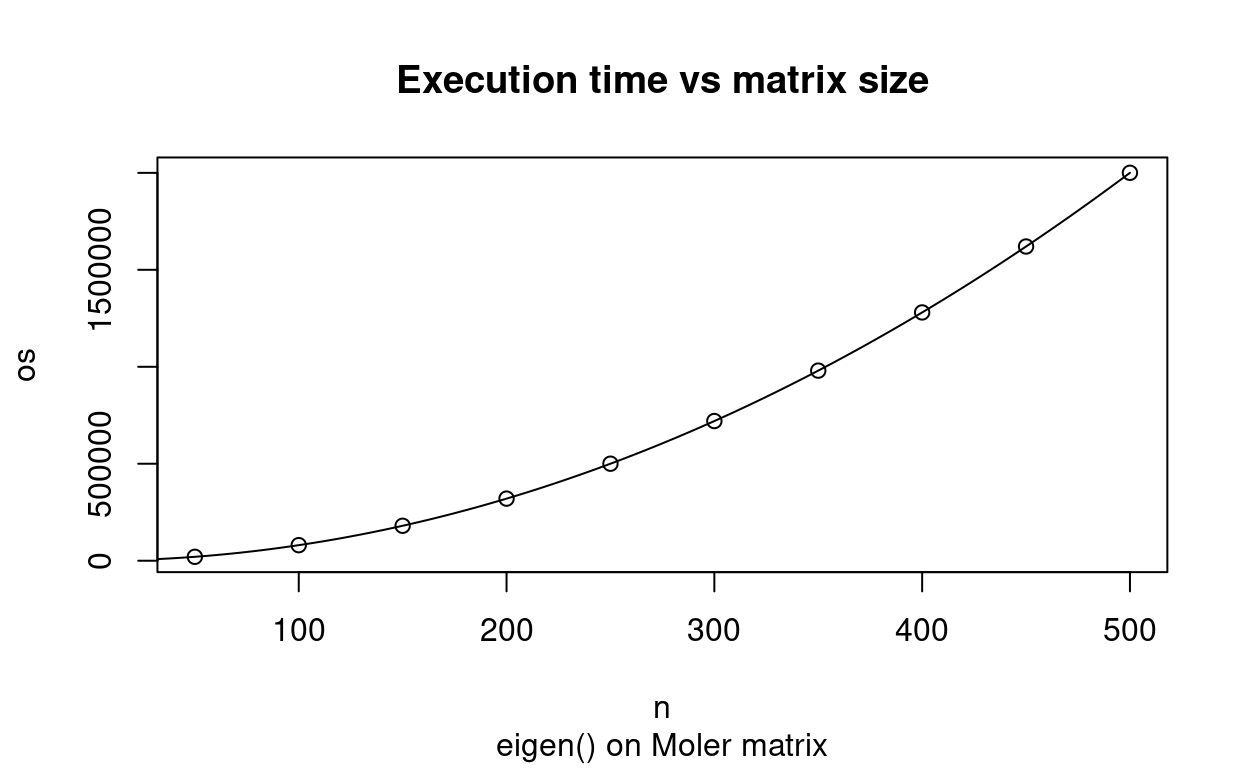
\includegraphics{RQtimes_files/figure-latex/drawtime2-1.pdf}

\subsection{Computing the Rayleigh Quotient}\label{computing-the-rayleigh-quotient}

The Rayleigh Quotient requires the quadratic form \(x' A x\) divided
by the inner product \(x' x\). R lets us form this in several ways.

\begin{verbatim}
rqdir<-function(x, AA){
  rq<-0.0
  n<-length(x) # assume x, AA conformable
  for (i in 1:n) {
     for (j in 1:n) {
        rq<-rq+x[i]*AA[[i,j]]*x[j] # Note - sign
     }
  }
  rq
}
\end{verbatim}

Somewhat better (as we shall show below) is

\begin{verbatim}
ray1<-function(x, AA){
    rq<-  t(x)%*%AA%*%x
}
\end{verbatim}

and (believed) better still is

\begin{verbatim}
ray2<-function(x, AA){
    rq<-  as.numeric(crossprod(x, crossprod(AA,x)))
}
\end{verbatim}

Note that we could implicitly include the minus sign in these
routines to allow for finding the maximal eigenvalue by minimizing
the Rayleigh Quotient of \(-A\). However, such shortcuts often rebound when
the implicit negation is overlooked.

If we already have the inner product \$ A x\$ as vector \texttt{ax} from some other
computation, then we can simply use

\begin{verbatim}
ray3<-function(x, AA, ax=axftn){
    # ax is a function to form AA%*%x 
    rq<- - as.numeric(crossprod(x, ax(x, AA)))
}
\end{verbatim}

\subsection{Matrix-vector products}\label{matrix-vector-products}

In generating the RQ, we do not actually need the matrix itself,
but simply the inner product with a vector \texttt{x\},\ from\ which\ \ a\ second\ inner\ produce\ with}x\} gives us the quadratic form
\$ x' A x\$. If \texttt{n\}\ is\ the\ order\ of\ the\ problem,\ then\ for\ large}n\}, we avoid storing and manipulating a very large matrix if
we use \B{implicit inner product} formation. We do this with the
following code. For future reference, we include the multiplication
by an identity.

\begin{verbatim}
ax<-function(x, AA){
   u<- as.numeric(AA%*%x)
}

axx<-function(x, AA){
   u<- as.numeric(crossprod(AA, x))
}
\end{verbatim}

Note that second argument, supposedly communicating the matrix which is
to be used in the matrix-vector product, is ignored in the following
implicit product routine. It is present only to provide a common syntax
when we wish to try different routines within other computations.

\begin{verbatim}
aximp<-function(x, AA=1){ # implicit moler A*x
   n<-length(x)
   y<-rep(0,n)
   for (i in 1:n){
      tt<-0.
      for (j in 1:n) {
          if (i == j) tt<-tt+i*x[i]
          else tt<-tt+(min(i,j) - 2)*x[j]
      }
      y[i]<-tt 
   }
   y
}
ident<-function(x, B=1) x # identity
\end{verbatim}

However, Ravi Varadhan has suggested the following vectorized code for
the implicit matrix-vector product.

\begin{verbatim}
axmolerfast <- function(x, AA=1) {
# A fast and memory-saving version of A%*%x  
# For Moler matrix. Note we need a matrix argument to match other functions
n <- length(x)
j <- 1:n
ax <- rep(0, n)
for (i in 1:n) {
term <- x * (pmin(i, j) - 2)
ax[i] <- sum(term[-i]) 
}
ax <- ax + j*x
ax
}
\end{verbatim}

We can also use external language routines, for example in Fortran.
However, this needs a Fortran \B{subroutine} which outputs the result as one of
the returned components. The subroutine is in file `moler.f\}.

\begin{verbatim}
      subroutine moler(n, x, ax)
      integer n, i, j
      double precision x(n), ax(n), sum
c     return ax = A * x for A = moler matrix
c     A[i,j]=min(i,j)-2 for i<>j, or i for i==j
      do 20 i=1,n
         sum=0.0
         do 10 j=1,n
            if (i.eq.j) then
               sum = sum+i*x(i)
            else
               sum = sum+(min(i,j)-2)*x(j)
            endif
 10      continue
         ax(i)=sum
 20   continue
      return
      end
\end{verbatim}

This is then compiled in a form suitable for R use by the command (this
is a command-line tool, and was run in Ubuntu Linux in a directory containing
the file \texttt{\{moler.f} but outside this vignette):

\begin{verbatim}
R CMD SHLIB moler.f
\end{verbatim}

This creates files \texttt{\{moler.o} and `\{moler.so\}, the latter being the
dynamically loadable library we need to bring into our R session.

\begin{verbatim}
dyn.load("moler.so")
cat("Is the mat multiply loaded? ",is.loaded("moler"),"\n")
\end{verbatim}

\begin{verbatim}
#> Is the mat multiply loaded?  TRUE
\end{verbatim}

\begin{verbatim}
axftn<-function(x, AA=1) { # ignore second argument
   n<-length(x) # could speed up by having this passed
   vout<-rep(0,n) # purely for storage
   res<-(.Fortran("moler", n=as.integer(n), x=as.double(x), vout=as.double(vout)))$vout
}
\end{verbatim}

We can also byte compile each of the routines above

Now it is possible to time the different approaches to the matrix-vector
product.

\begin{verbatim}
dyn.load("moler.so")
cat("Is the mat multiply loaded? ",is.loaded("moler"),"\n")
\end{verbatim}

\begin{verbatim}
#> Is the mat multiply loaded?  TRUE
\end{verbatim}

\begin{verbatim}
require(microbenchmark)
nmax<-10
ptable<-matrix(NA, nrow=nmax, ncol=6) # to hold results
# loop over sizes
for (ni in 1:nmax){
  n<-50*ni
  x<-runif(n) # generate a vector 
  ptable[[ni, 1]]<-n
  AA<-molermat(n)
  tax<-system.time(oax<-replicate(100,ax(x, AA))[,1])[[1]]
  taxx<-system.time(oaxx<-replicate(100,axx(x, AA))[,1])[[1]]
  if (! identical(oax, oaxx)) stop("oaxx NOT correct")
  taxftn<-system.time(oaxftn<-replicate(100,axftn(x, AA=1))[,1])[[1]]
  if (! identical(oax, oaxftn)) stop("oaxftn NOT correct")
  taximp<-system.time(oaximp<-replicate(100,aximp(x, AA=1))[,1])[[1]]
  if (! identical(oax, oaximp)) stop("oaximp NOT correct")
  taxmfi<-system.time(oaxmfi<-replicate(100,axmolerfast(x, AA=1))[,1])[[1]]
  if (! identical(oax, oaxmfi)) stop("oaxmfi NOT correct")
  ptable[[ni, 2]]<-tax
  ptable[[ni, 3]]<-taxx
  ptable[[ni, 4]]<-taxftn
  ptable[[ni, 5]]<-taximp
  ptable[[ni, 6]]<-taxmfi
}

axtym<-data.frame(n=ptable[,1], ax=ptable[,2], axx=ptable[,3],  axftn=ptable[,4], 
                  aximp=ptable[,5], axmfast=ptable[,6])
print(axtym)
\end{verbatim}

\begin{verbatim}
#>      n    ax   axx axftn  aximp axmfast
#> 1   50 0.000 0.000 0.001  0.125   0.037
#> 2  100 0.003 0.006 0.013  0.508   0.071
#> 3  150 0.016 0.000 0.010  1.124   0.116
#> 4  200 0.003 0.005 0.044  2.025   0.162
#> 5  250 0.014 0.018 0.061  3.103   0.216
#> 6  300 0.052 0.005 0.082  4.467   0.266
#> 7  350 0.031 0.022 0.114  6.135   0.331
#> 8  400 0.032 0.025 0.127  7.931   0.388
#> 9  450 0.016 0.033 0.138 10.164   0.456
#> 10 500 0.038 0.052 0.159 12.445   0.523
\end{verbatim}

From the above output, we see that the \texttt{crossprod} variant of the
matrix-vector product appears to be the fastest. However, we have omitted
the time to build the matrix. If we must build the matrix, then we need
somehow to include that time. Because the times for the matrix-vector
product were so short, we used \texttt{replicate\}\ above\ to\ run\ 100\ copies\ \ of\ the\ same\ calculation,\ which\ may\ give\ some\ distortion\ of\ the\ timings.\ However,\ we\ believe\ the\ scale\ of\ the\ times\ is\ more\ or\ less\ correct.\ To\ \ compare\ these\ times\ to\ the\ times\ for\ the\ Fortran\ or\ implicit\ matrix-vector\ routines,\ we\ should\ add\ a\ multiple\ of\ the\ relevant\ interpreted\ or\ compiled\ build\ times.\ Here\ we\ have\ used\ the\ times\ for\ the\ rather\ poor}molermat()\} function, but this is simply to illustrate the range
of potential timings. Apportioning such ``fixed costs'' to timings is
never a trivial decision. Similarly if, where and how to store
large matrices if we do build them, and whether it is worth building
them more than once if storage is an issue, are all questions that
may need to be addressed if performance becomes important.

\begin{verbatim}
adjtym<-data.frame(n=axtym$n, axx1=axtym$axx+1*bmattym$buildi, 
     axxz=axtym$axx+100*bmattym$buildi, 
     axftn=axtym$axftn, aximp=axtym$aximp)
print(adjtym)
\end{verbatim}

\begin{verbatim}
#>      n      axx1      axxz axftn  aximp
#> 1   50  4628.746  462874.6 0.001  0.125
#> 2  100  5978.380  597837.4 0.013  0.508
#> 3  150 10136.813 1013681.3 0.010  1.124
#> 4  200 16038.074 1603806.9 0.044  2.025
#> 5  250 24331.520 2433150.2 0.061  3.103
#> 6  300 34352.869 3435286.4 0.082  4.467
#> 7  350 45955.674 4595565.3 0.114  6.135
#> 8  400 58745.996 5874597.1 0.127  7.931
#> 9  450 77464.626 7746459.3 0.138 10.164
#> 10 500 91165.558 9116550.7 0.159 12.445
\end{verbatim}

Out of all this, we see that the Fortran implicit matrix-vector product is
the overall winner at all values of \texttt{n}. Moreover, it does NOT
require the creation and storage of the matrix. However, using Fortran
does involve rather more work for the user, and for most applications
it is likely we could live with the use of either

\begin{itemize}
\tightlist
\item
  the interpreted matrix-product based on \texttt{crossprod}
  and an actual matrix is good enough, especially if a fast
  matrix build is used and we have plenty of memory, or
\item
  the interpreted or byte-code compiled implicit matrix-vector
  multiply \texttt{axmolerfast}.
\end{itemize}

\subsection{RQ computation times\}}\label{rq-computation-times}

We have in Ref\{sect:crq\} set up three versions of a Rayleigh
Quotient calculation in addition to the direct form. The third
form is set up to use the \code{axftn} routine that we have
already shown is efficient. We could also use this with the
implicit matrix-vector product \code{axmolerfast}.

It seems overkill to show the RQ computation time for all versions
and matrices, so we will do the timing simply for a matrix of
order 500.

\begin{verbatim}
dyn.load("moler.so")
  n<-500
  x<-runif(n) # generate a vector 
  AA<-molermat(n)
  tdi<-microbenchmark(rdi<-rqdir(x, AA))$time
  cat("Direct algorithm: ",mean(tdi)*0.001,"\n")
\end{verbatim}

\begin{verbatim}
#> Direct algorithm:  17287.62
\end{verbatim}

\begin{verbatim}
  t1i<-microbenchmark(r1i<-ray1(x, AA))$time
  cat("ray1: mat-mult algorithm: ", mean(t1i)*0.001,"\n")
\end{verbatim}

\begin{verbatim}
#> ray1: mat-mult algorithm:  151.8565
\end{verbatim}

\begin{verbatim}
  t2i<-microbenchmark(r2i<-ray2(x, AA))$time
  cat("ray2: crossprod algorithm: ",mean(t2i)*0.001,"\n")
\end{verbatim}

\begin{verbatim}
#> ray2: crossprod algorithm:  140.0596
\end{verbatim}

\begin{verbatim}
  t3fi<-microbenchmark(r3i<-ray3(x, AA, ax=axftn))$time
  cat("ray3: ax Fortran + crossprod: ",mean(t3fi)*0.001,"\n")
\end{verbatim}

\begin{verbatim}
#> ray3: ax Fortran + crossprod:  661.0016
\end{verbatim}

\begin{verbatim}
  t3ri<-microbenchmark(r3i<-ray3(x, AA, ax=axmolerfast))$time
  cat("ray3: ax fast R implicit + crossprod: ",mean(t3ri)*0.001,"\n")
\end{verbatim}

\begin{verbatim}
#> ray3: ax fast R implicit + crossprod:  5639.364
\end{verbatim}

Here we see that the use of the \texttt{crossprod} in \texttt{ray2} is
very fast, and this is interpreted code. Once again, we note that all
timings except those for \texttt{ray3} should have some adjustment for
the building of the matrix. If storage is an issue, then \texttt{ray3},
which uses the implicit matrix-vector product in Fortran, is the
approach of choice. My own preference would be to use this option
if the Fortran matrix-vector product subroutine is already available
for the matrix required. I would not, however, generally choose to
write the Fortran subroutine for a ``new'' problem matrix. The fast
implicit matrix-vector tool with \texttt{ray3} is also useful and
quite fast if we need to minimize memory use.

\section{References}\label{references}

\bibliography{../sumscale.bib}

\address{%
John C. Nash\\
retired professor, University of Ottawa\\%
Telfer School of Management\\ Ottawa ON Canada K1N 6N5\\
%
%
\textit{ORCiD: \href{https://orcid.org/0000-0002-2762-8039}{0000-0002-2762-8039}}\\%
\href{mailto:profjcnash@gmail.com}{\nolinkurl{profjcnash@gmail.com}}%
}
